\documentclass[12pt]{book}

%For sending to printer such as lulu/createsace, search for %PRINT

%See text for 
%FIXMEevillayouthack
% for evil layout hacks

%\usepackage{pdf14}
%Paper saving
%\documentclass[12pt,openany]{book}
%\documentclass[10pt,openany]{book}
%\documentclass[8pt,openany]{extbook}
%if using smaller font you should also rerun the figures,
% that is in figures/ run run-all-xp.sh (must have epix installed)

\usepackage[T1]{fontenc}

% Footnotes should use symbols, not numbers.  Numbered footnotes are
% evil
\usepackage[perpage,symbol*]{footmisc}

\usepackage[shortlabels]{enumitem}
\usepackage{ifpdf}
\usepackage{amsmath}
\usepackage{amsfonts}
\usepackage{amssymb}
\usepackage{amsthm}
\usepackage{graphicx}
\usepackage{color}

% Remove page numbers on chapter opens
% must come before fullpage
\usepackage{nopageno}

\usepackage[headings]{fullpage}

% smaller margins top/bottom margins
\addtolength{\textheight}{0.8in}
\addtolength{\topmargin}{-0.3in}

%PRINT
%First offset even/odd pages a bit
%\addtolength{\oddsidemargin}{0.2in}
%\addtolength{\evensidemargin}{-0.2in}

%PRINT
%Now cut page size a bit.  I'll run it through ghostcript anyway
%to convert to the right size, but this is good for crown quatro
%conversion, don't use for the full letter size versions
%\addtolength{\paperwidth}{-0.3in}
%\addtolength{\paperheight}{-1in}
%\addtolength{\topmargin}{-0.5in}
%\addtolength{\oddsidemargin}{-0.15in}
%\addtolength{\evensidemargin}{-0.15in}


\usepackage{varioref}
\usepackage{imakeidx}
\PassOptionsToPackage{hyphens}{url}
\usepackage{hyperref} % do NOT set [ocgcolorlinks] here!

%If you have an older tex installation you might need
%to comment out the next line:
%PRINT for a printer (lulu/createspace) run without
\usepackage[ocgcolorlinks]{ocgx2}

%\usepackage[all]{hypcap} %handled by caption
\usepackage[shortalphabetic]{amsrefs}
\usepackage{nicefrac}
\usepackage{microtype}
\usepackage{import}

\usepackage{draftwatermark}
\SetWatermarkText{Draft of v5.0 as of \today. May change substantially!}
\SetWatermarkAngle{90}
\SetWatermarkHorCenter{0.5in}
\SetWatermarkColor[gray]{0.7}
\SetWatermarkScale{0.18}

\usepackage[margin=10pt,font=small,labelfont=bf,labelsep=colon,singlelinecheck=false]{caption}

\usepackage{tikz}
\usetikzlibrary{cd}
%\usepackage{rotating}

\usepackage{cellspace}
\usepackage[toc,nopostdot,sort=use,nomain,automake]{glossaries}

\usepackage{vogtwidebar}

%%%
%NOTE: If changing fonts, also change fonts in figures/run-xp-topdf.sh
% AND then rerun run-all-xp.sh (must have epix installed)
%%%
% Times
%\usepackage{txfonts}
% Times, but symbol/cm/ams math fonts
\usepackage{mathptmx}
% But we do want helvetica for sans
\usepackage{helvet}

%enumitem global options
\setlist{leftmargin=*,itemsep=0.5\itemsep,parsep=0.5\parsep,topsep=0.5\topsep,partopsep=0.5\partopsep}

\newenvironment{myfigureht}{%
\begin{figure}[h!t]
\noindent\rule{\textwidth}{0.4pt}\vspace{12pt}\par\centering}%
{\par\noindent\rule{\textwidth}{0.4pt}
\end{figure}}

% useful
\newcommand{\ignore}[1]{}

% analysis/geometry stuff
\newcommand{\ann}{\operatorname{ann}}
\renewcommand{\Re}{\operatorname{Re}}
\renewcommand{\Im}{\operatorname{Im}}
\newcommand{\Orb}{\operatorname{Orb}}
\newcommand{\hol}{\operatorname{hol}}
\newcommand{\aut}{\operatorname{aut}}
\newcommand{\codim}{\operatorname{codim}}
\newcommand{\sing}{\operatorname{sing}}

% reals
\newcommand{\esssup}{\operatorname{ess~sup}}
\newcommand{\essran}{\operatorname{essran}}
\newcommand{\innprod}[2]{\langle #1 | #2 \rangle}
\newcommand{\linnprod}[2]{\langle #1 , #2 \rangle}
\newcommand{\supp}{\operatorname{supp}}
\newcommand{\Nul}{\operatorname{Nul}}
\newcommand{\Ran}{\operatorname{Ran}}
\newcommand{\sabs}[1]{\lvert {#1} \rvert}
\newcommand{\snorm}[1]{\lVert {#1} \rVert}
\newcommand{\abs}[1]{\left\lvert {#1} \right\rvert}
\newcommand{\norm}[1]{\left\lVert {#1} \right\rVert}

% sets (some)
\newcommand{\C}{{\mathbb{C}}}
\newcommand{\R}{{\mathbb{R}}}
\newcommand{\Z}{{\mathbb{Z}}}
\newcommand{\N}{{\mathbb{N}}}
\newcommand{\Q}{{\mathbb{Q}}}
\newcommand{\D}{{\mathbb{D}}}
\newcommand{\F}{{\mathbb{F}}}

% consistent
\newcommand{\bB}{{\mathbb{B}}}
\newcommand{\bC}{{\mathbb{C}}}
\newcommand{\bR}{{\mathbb{R}}}
\newcommand{\bZ}{{\mathbb{Z}}}
\newcommand{\bN}{{\mathbb{N}}}
\newcommand{\bQ}{{\mathbb{Q}}}
\newcommand{\bD}{{\mathbb{D}}}
\newcommand{\bF}{{\mathbb{F}}}
\newcommand{\bH}{{\mathbb{H}}}
\newcommand{\bO}{{\mathbb{O}}}
\newcommand{\bP}{{\mathbb{P}}}
\newcommand{\bK}{{\mathbb{K}}}
\newcommand{\bV}{{\mathbb{V}}}
\newcommand{\CP}{{\mathbb{CP}}}
\newcommand{\RP}{{\mathbb{RP}}}
\newcommand{\HP}{{\mathbb{HP}}}
\newcommand{\OP}{{\mathbb{OP}}}
\newcommand{\sA}{{\mathcal{A}}}
\newcommand{\sB}{{\mathcal{B}}}
\newcommand{\sC}{{\mathcal{C}}}
\newcommand{\sF}{{\mathcal{F}}}
\newcommand{\sG}{{\mathcal{G}}}
\newcommand{\sH}{{\mathcal{H}}}
\newcommand{\sM}{{\mathcal{M}}}
\newcommand{\sO}{{\mathcal{O}}}
\newcommand{\sP}{{\mathcal{P}}}
\newcommand{\sQ}{{\mathcal{Q}}}
\newcommand{\sR}{{\mathcal{R}}}
\newcommand{\sS}{{\mathcal{S}}}
\newcommand{\sI}{{\mathcal{I}}}
\newcommand{\sL}{{\mathcal{L}}}
\newcommand{\sK}{{\mathcal{K}}}
\newcommand{\sU}{{\mathcal{U}}}
\newcommand{\sV}{{\mathcal{V}}}
\newcommand{\sX}{{\mathcal{X}}}
\newcommand{\sY}{{\mathcal{Y}}}
\newcommand{\sZ}{{\mathcal{Z}}}
\newcommand{\fS}{{\mathfrak{S}}}

\newcommand{\interior}{\operatorname{int}}

% Topo stuff
\newcommand{\id}{\textit{id}}
\newcommand{\im}{\operatorname{im}}
\newcommand{\rank}{\operatorname{rank}}
\newcommand{\Tor}{\operatorname{Tor}}
\newcommand{\Torsion}{\operatorname{Torsion}}
\newcommand{\Ext}{\operatorname{Ext}}
\newcommand{\Hom}{\operatorname{Hom}}

%extra thingies
\newcommand{\mapsfrom}{\ensuremath{\text{\reflectbox{$\mapsto$}}}}
\newcommand{\from}{\ensuremath{\leftarrow}}
\newcommand{\dhat}[1]{\hat{\hat{#1}}}
\newcommand{\spn}{\operatorname{span}}

% San Serif fonts
%\renewcommand{\familydefault}{\sfdefault}

% To allow skrinking to 5.5 x 8.5 inches without whitespaces
% Make sure to rerun makeindex and makeglossaries as well
% Useful for printing on lulu.com and saving on paper
%\addtolength{\textheight}{2.13in}
%\addtolength{\paperheight}{2.13in}

\definecolor{mypersianblue}{rgb}{0.11, 0.22, 0.73}

\hypersetup{
    pdfborderstyle={/S/U/W 0.5}, %this just in case ocg isn't there
    citecolor=mypersianblue,
    filecolor=mypersianblue,
    linkcolor=mypersianblue,
    urlcolor=mypersianblue,
    pdfkeywords={real analysis, Riemann integral, derivative, limit, sequence},
    pdfsubject={Real Analysis},
    pdftitle={Basic Analysis: Introduction to Real Analysis},
    pdfauthor={Jiri Lebl}
}

% Set up our index
\makeindex

% Very simple indexing
\newcommand{\myindex}[1]{#1\index{#1}}

% define this to be empty to kill notes
\newcommand{\sectionnotes}[1]{\noindent \emph{Note: #1} \medskip \par}

% Define this to be empty to not skip page before the sections to
% save some paper
\newcommand{\sectionnewpage}{\clearpage}
%\newcommand{\sectionnewpage}{}

\author{Ji\v{r}\'i Lebl}

\title{Basic Analysis: Introduction to Real Analysis}

% Don't include subsections
\setcounter{tocdepth}{1}

\theoremstyle{plain}
\newtheorem{thm}{Theorem}[section]
\newtheorem{lemma}[thm]{Lemma}
\newtheorem{prop}[thm]{Proposition}
\newtheorem{cor}[thm]{Corollary}

\theoremstyle{remark}
\newtheorem{remark}[thm]{Remark}

\theoremstyle{definition}
\newtheorem{defn}[thm]{Definition}

\newtheoremstyle{exercise}% name
  {}% Space above
  {}% Space below
  {\itshape \small}% Body font
  {}% Indent amount 1
  {\bfseries \itshape \small}% Theorem head font
  {:}% Punctuation after theorem head
  {.5em}% Space after theorem head 2
  {}% Theorem head spec (can be left empty, meaning "normal")

\newenvironment{exnote}{\small}{}

\theoremstyle{exercise}
\newtheorem{exercise}{Exercise}[section]

\newtheoremstyle{example}% name
  {}% Space above
  {}% Space below
  {}% Body font
  {}% Indent amount 1
  {\bfseries}% Theorem head font
  {:}% Punctuation after theorem head
  {.5em}% Space after theorem head 2
  {}% Theorem head spec (can be left empty, meaning "normal")

\theoremstyle{example}
\newtheorem{example}[thm]{Example}

% referencing
\newcommand{\figureref}[1]{\hyperref[#1]{Figure~\ref*{#1}}}
\newcommand{\tableref}[1]{\hyperref[#1]{Table~\ref*{#1}}}
\newcommand{\chapterref}[1]{\hyperref[#1]{chapter~\ref*{#1}}}
\newcommand{\Chapterref}[1]{\hyperref[#1]{Chapter~\ref*{#1}}}
\newcommand{\sectionref}[1]{\hyperref[#1]{\S\ref*{#1}}}
\newcommand{\exerciseref}[1]{\hyperref[#1]{Exercise~\ref*{#1}}}
\newcommand{\remarkref}[1]{\hyperref[#1]{Remark~\ref*{#1}}}
\newcommand{\exampleref}[1]{\hyperref[#1]{Example~\ref*{#1}}}
\newcommand{\thmref}[1]{\hyperref[#1]{Theorem~\ref*{#1}}}
\newcommand{\propref}[1]{\hyperref[#1]{Proposition~\ref*{#1}}}
\newcommand{\lemmaref}[1]{\hyperref[#1]{Lemma~\ref*{#1}}}
\newcommand{\corref}[1]{\hyperref[#1]{Corollary~\ref*{#1}}}
\newcommand{\defnref}[1]{\hyperref[#1]{Definition~\ref*{#1}}}


% List of Symbols/Notation
\newglossary[nlg]{notation}{not}{ntn}{List of Notation}

\loadglsentries{notations}
\makeglossaries


\begin{document}

\ifpdf
  \pdfbookmark{Title Page}{title}
\fi
\newlength{\centeroffset}
\setlength{\centeroffset}{-0.5\oddsidemargin}
\addtolength{\centeroffset}{0.5\evensidemargin}
%\addtolength{\textwidth}{-\centeroffset}
\thispagestyle{empty}
\vspace*{\stretch{1}}
\noindent\hspace*{\centeroffset}\makebox[0pt][l]{\begin{minipage}{\textwidth}
\flushright
{\Huge\bfseries \sffamily Basic Analysis }
\noindent\rule[-1ex]{\textwidth}{5pt}\\[2.5ex]
\hfill\emph{\Large \sffamily Introduction to Real Analysis, Volume I}
\end{minipage}}

\vspace{\stretch{1}}
\noindent\hspace*{\centeroffset}\makebox[0pt][l]{\begin{minipage}{\textwidth}
\flushright
{\bfseries 
by Ji{\v r}\'i Lebl\\[3ex]} 
\today
\\
(version 5.0 unfinished)
% --- 5th edition, 0th update)
\end{minipage}}

%\addtolength{\textwidth}{\centeroffset}
\vspace{\stretch{2}}


\pagebreak

\vspace*{\fill}

\noindent
Typeset in \LaTeX.


\bigskip

\noindent
Copyright \copyright 2009--2018 Ji{\v r}\'i Lebl

%\noindent
%ISBN XXXX

\bigskip

\noindent

\includegraphics[width=1.38in]{figures/license}
\quad
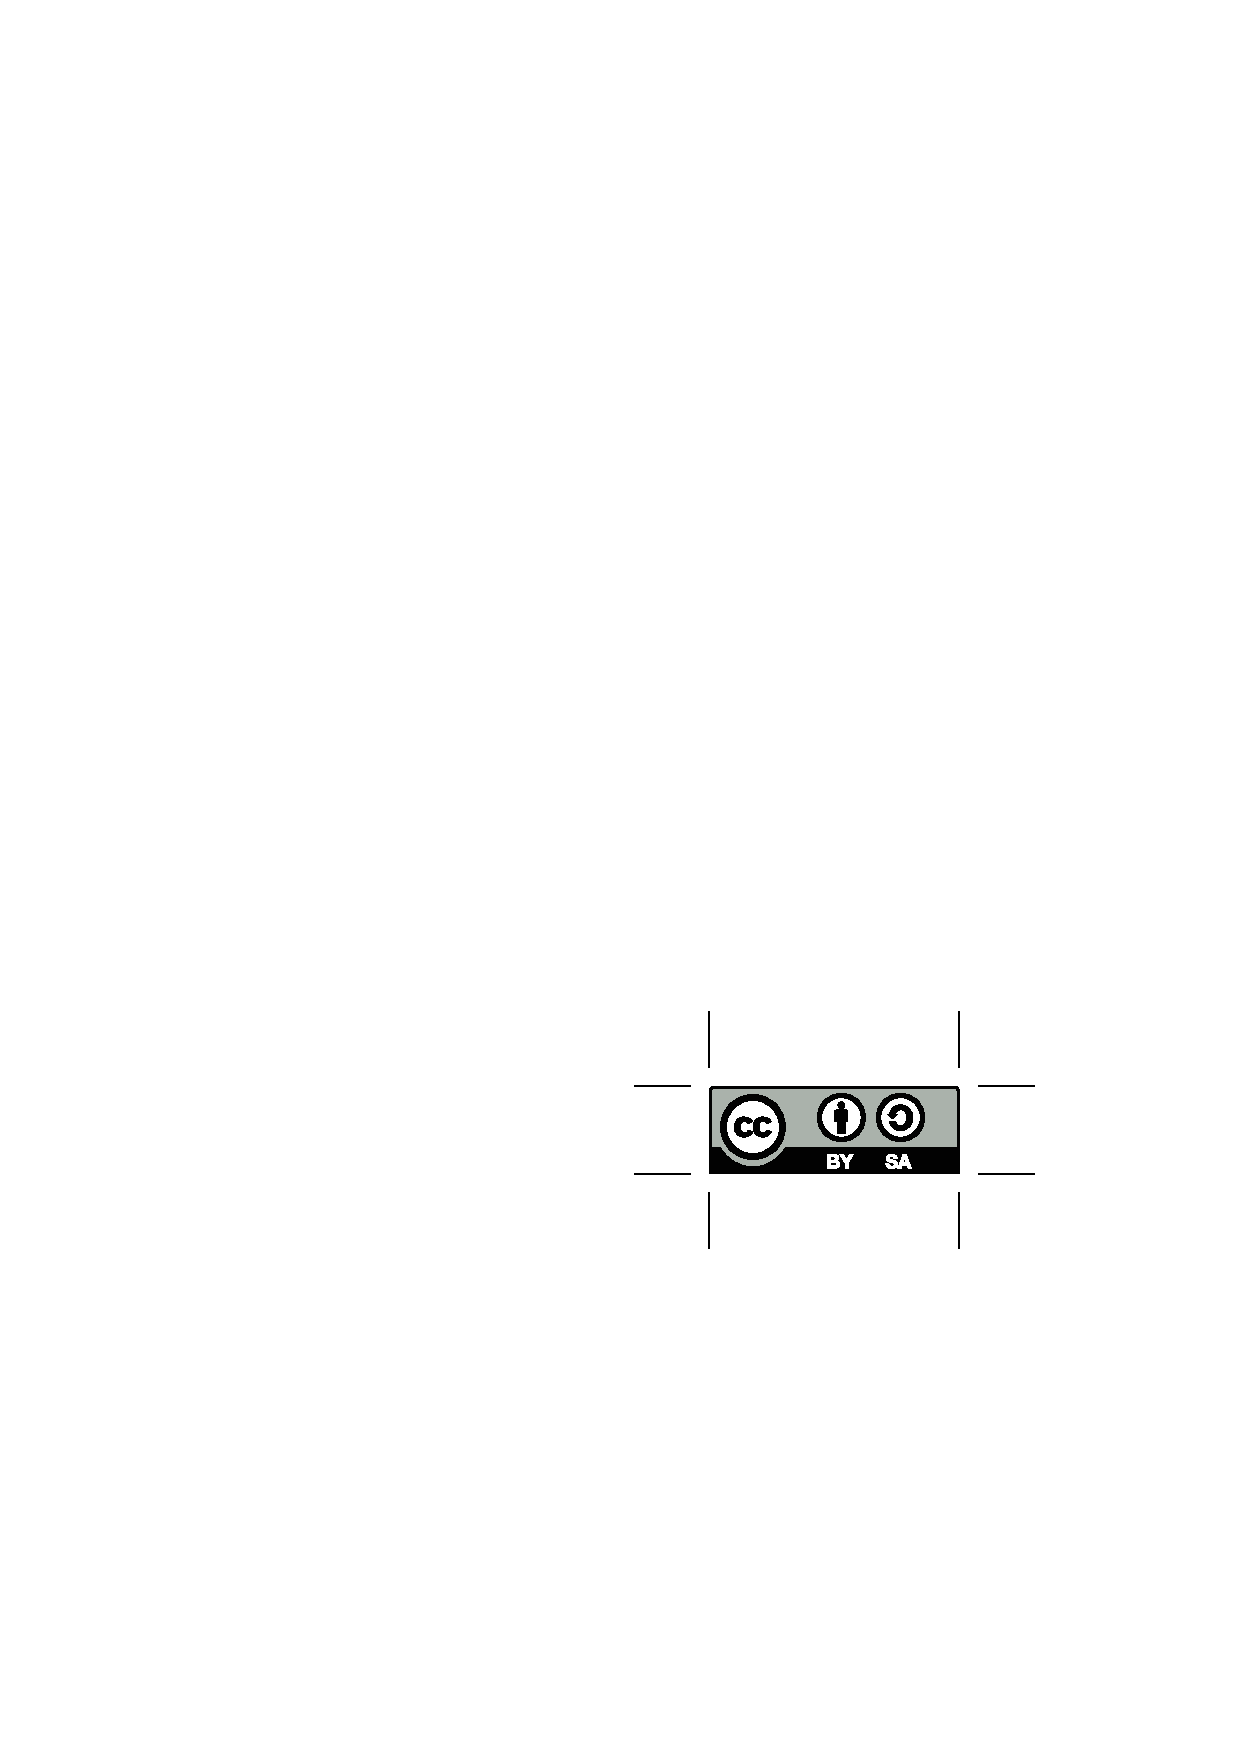
\includegraphics[width=1.38in]{figures/license2}

\bigskip

\noindent
This work is dual licensed under
the Creative Commons
Attribution-Non\-commercial-Share Alike 4.0 International License and
the Creative Commons
Attribution-Share Alike 4.0 International License.
To view a
copy of these licenses, visit
\url{http://creativecommons.org/licenses/by-nc-sa/4.0/}
or
\url{http://creativecommons.org/licenses/by-sa/4.0/}
or send a letter to
Creative Commons
PO Box 1866, Mountain View, CA 94042, USA.

\bigskip

\noindent
You can use, print, duplicate, share this book as much as you want.  You can
base your own notes on it and reuse parts if you keep the license the
same.  You can assume the license is either the CC-BY-NC-SA or CC-BY-SA,
whichever is compatible with what you wish to do, your derivative works must
use at least one of the licenses.

\bigskip

\noindent
During the writing of these notes, 
the author was in part supported by NSF grants DMS-0900885 and
DMS-1362337.

\bigskip

\noindent
The date is the main identifier of version.  The major version / edition
number is raised only if there have been substantial changes.  Edition
number started at 4, that is, version 4.0, as it was not kept track of
before.  %The edition given with the ISBN number is the major version.

\bigskip

\noindent
See \url{http://www.jirka.org/ra/} for more information
(including contact information).


% For large print do this
%\large

\microtypesetup{protrusion=false}
\tableofcontents
\microtypesetup{protrusion=true}

\newpage

%%%%%%%%%%%%%%%%%%%%%%%%%%%%%%%%%%%%%%%%%%%%%%%%%%%%%%%%%%%%%%%%%%%%%%%%%%%%%%

% Introduction to Volume 1
\input ch-vol1-intro.tex

%%%%%%%%%%%%%%%%%%%%%%%%%%%%%%%%%%%%%%%%%%%%%%%%%%%%%%%%%%%%%%%%%%%%%%%%%%%%%%

% Real Numbers chapter
\input ch-real-nums.tex

%%%%%%%%%%%%%%%%%%%%%%%%%%%%%%%%%%%%%%%%%%%%%%%%%%%%%%%%%%%%%%%%%%%%%%%%%%%%%%

% Sequences and Series chapter
\input ch-seq-ser.tex

%%%%%%%%%%%%%%%%%%%%%%%%%%%%%%%%%%%%%%%%%%%%%%%%%%%%%%%%%%%%%%%%%%%%%%%%%%%%%%

% Continuous Functions chapter
\input ch-contfunc.tex

%%%%%%%%%%%%%%%%%%%%%%%%%%%%%%%%%%%%%%%%%%%%%%%%%%%%%%%%%%%%%%%%%%%%%%%%%%%%%%

% The Derivative chapter
\input ch-der.tex

%%%%%%%%%%%%%%%%%%%%%%%%%%%%%%%%%%%%%%%%%%%%%%%%%%%%%%%%%%%%%%%%%%%%%%%%%%%%%%

% The Riemann Integral chapter
\input ch-riemann.tex

%%%%%%%%%%%%%%%%%%%%%%%%%%%%%%%%%%%%%%%%%%%%%%%%%%%%%%%%%%%%%%%%%%%%%%%%%%%%%%

% Sequences of Functions chapter
\input ch-seq-funcs.tex

%%%%%%%%%%%%%%%%%%%%%%%%%%%%%%%%%%%%%%%%%%%%%%%%%%%%%%%%%%%%%%%%%%%%%%%%%%%%%%

% Metric Spaces chapter
\input ch-metric.tex

%%%%%%%%%%%%%%%%%%%%%%%%%%%%%%%%%%%%%%%%%%%%%%%%%%%%%%%%%%%%%%%%%%%%%%%%%%%%%%
%%%%%%%%%%%%%%%%%%%%%%%%%%%%%%%%%%%%%%%%%%%%%%%%%%%%%%%%%%%%%%%%%%%%%%%%%%%%%%
%%%%%%%%%%%%%%%%%%%%%%%%%%%%%%%%%%%%%%%%%%%%%%%%%%%%%%%%%%%%%%%%%%%%%%%%%%%%%%

\cleardoublepage  
\phantomsection
\addcontentsline{toc}{chapter}{Further Reading}
\markboth{FURTHER READING}{FURTHER READING}
\begin{bibchapter}[Further Reading]
\begin{biblist}[\normalsize]

\bib{BS}{book}{
   author={Bartle, Robert G.},
   author={Sherbert, Donald R.},
   title={Introduction to real analysis},
   edition={3},
   publisher={John Wiley \& Sons Inc.},
   place={New York},
   date={2000},
}

\bib{DW}{book}{
   author={D'Angelo, John P.},
   author={West, Douglas B.},
   title={Mathematical Thinking: Problem-Solving and Proofs},
   edition={2},
   publisher={Prentice Hall},
   date={1999},
}

\bib{GIAM}{misc}{
   author={Fields, Joseph E.},
   title={A Gentle Introduction to the Art of Mathematics},
   note={Available at \url{http://giam.southernct.edu/GIAM/}},
}

\bib{Hammack}{misc}{
   author={Hammack, Richard},
   title={Book of Proof},
   note={Available at \url{http://www.people.vcu.edu/~rhammack/BookOfProof/}},
}

\bib{Rosenlicht}{book}{
   author={Rosenlicht, Maxwell},
   title={Introduction to analysis},
   note={Reprint of the 1968 edition},
   publisher={Dover Publications Inc.},
   place={New York},
   date={1986},
   pages={viii+254},
   isbn={0-486-65038-3},
}

\bib{Rudin:baby}{book}{
   author={Rudin, Walter},
   title={Principles of mathematical analysis},
   edition={3},
   note={International Series in Pure and Applied Mathematics},
   publisher={McGraw-Hill Book Co.},
   place={New York},
   date={1976},
   pages={x+342},
}

\bib{Trench}{book}{
   author={Trench, William F.},
   title={Introduction to real analysis},
   year={2003},
   publisher={Pearson Education},
   note={\url{http://ramanujan.math.trinity.edu/wtrench/texts/TRENCH_REAL_ANALYSIS.PDF}},
}



\end{biblist}
\end{bibchapter}

%%%%%%%%%%%%%%%%%%%%%%%%%%%%%%%%%%%%%%%%%%%%%%%%%%%%%%%%%%%%%%%%%%%%%%%%%%%%%%
%%%%%%%%%%%%%%%%%%%%%%%%%%%%%%%%%%%%%%%%%%%%%%%%%%%%%%%%%%%%%%%%%%%%%%%%%%%%%%
%%%%%%%%%%%%%%%%%%%%%%%%%%%%%%%%%%%%%%%%%%%%%%%%%%%%%%%%%%%%%%%%%%%%%%%%%%%%%%

\cleardoublepage
\phantomsection
\addcontentsline{toc}{chapter}{\indexname}  
\printindex

%%%%%%%%%%%%%%%%%%%%%%%%%%%%%%%%%%%%%%%%%%%%%%%%%%%%%%%%%%%%%%%%%%%%%%%%%%%%%%
%%%%%%%%%%%%%%%%%%%%%%%%%%%%%%%%%%%%%%%%%%%%%%%%%%%%%%%%%%%%%%%%%%%%%%%%%%%%%%
%%%%%%%%%%%%%%%%%%%%%%%%%%%%%%%%%%%%%%%%%%%%%%%%%%%%%%%%%%%%%%%%%%%%%%%%%%%%%%

%
% automake on glossaries doesn't work if the index is before the glossary.
% That's why the List of Notation is last, no other reason.  Problem is
% that printindex does a clearpage which screws up the delayed write18
% that glossaries sets up
%

\begingroup
\renewcommand{\pagelistname}{Page}
\setglossarystyle{long3colheader}
% correctly set up with cellspace
\renewenvironment{theglossary}%
  {\setlength\cellspacetoplimit{4pt}
   \setlength\cellspacebottomlimit{4pt}
   \setlength\LTleft{0pt}
   \setlength\LTright{0pt}
   \markboth{LIST OF NOTATION}{LIST OF NOTATION}
   \begin{longtable}{Sl @{\extracolsep{\fill}} Sl @{\extracolsep{\fill}} Sl}}%
  {\end{longtable}}%
\cleardoublepage
\printglossary[type=notation] 
\endgroup

\end{document}
